\documentclass[letterpaper]{article} % DO NOT CHANGE THIS
\usepackage[submission]{aaai2027}  % DO NOT CHANGE THIS
\usepackage[hyphens]{url}  % DO NOT CHANGE THIS
\usepackage{graphicx} % DO NOT CHANGE THIS
\urlstyle{rm} % DO NOT CHANGE THIS
\def\UrlFont{\rm}  % DO NOT CHANGE THIS
\usepackage{natbib}  % DO NOT CHANGE THIS AND DO NOT ADD ANY OPTIONS TO IT
\usepackage{caption} % DO NOT CHANGE THIS AND DO NOT ADD ANY OPTIONS TO IT
\frenchspacing  % DO NOT CHANGE THIS
\usepackage{booktabs}
\usepackage{amsmath}
\pdfinfo{
/TemplateVersion (2027.1)
}

\setcounter{secnumdepth}{1}

\title{Compressed, Not Mis-Scaled: The Structure of Metric Errors\\in Frozen Vision-Language Models}
\author{
    Anonymous Submission
}
\affiliations{
}

\begin{document}

\maketitle

\begin{abstract}
Vision-language models (VLMs) answer metric spatial questions poorly, and a common assumption is that they lack a sense of the absolute scale of the scene. We test this assumption on VSI-Bench with frozen Qwen3-VL models. We split the log-error of every answer into three parts: a systematic part that depends on the true magnitude, a part shared by all questions about the same scene, and a per-question remainder. The scene-shared part is small (at most 9\% of the variance), and correcting each scene by its own mean error lowers accuracy. Instead, answers are compressed toward typical values: short distances and small rooms are overestimated and long distances and large rooms are underestimated, with a log-log slope of about 0.5, while object sizes are nearly proportional. In line with this structure, no scale cue added to the prompt improves accuracy, whether it is a metric depth estimate, a learned scale, or the true size of another object in the scene. Answers move in the direction of the cue, but with a mean elasticity of at most 0.05, so doubling the cue changes the answer by a few percent. A positive control shows that the model can use numbers in the prompt: a stated correct answer raises accuracy by up to 50 points, and for room size the model copies the stated value at any scale. For distance and object size, however, it keeps most of its own estimate even against a stated answer that is off by a factor of two. Even ideal use of the object-size cue lowers accuracy. Scene scale is therefore not the missing ingredient: better metric answers require reducing compression and per-question error.
\end{abstract}

\section{Introduction}

\begin{figure*}[t]
\centering
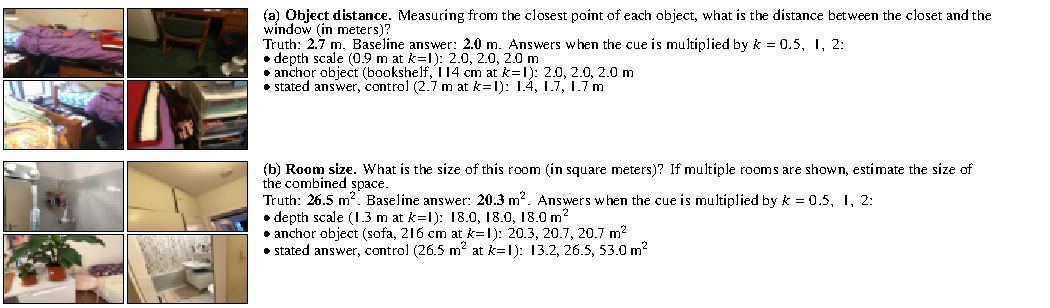
\includegraphics[width=\textwidth]{fig_teaser.pdf}
\caption{Scale cues barely change metric answers, even when exact. Typical behavior of Qwen3-VL-4B on two evaluation questions (four of the 16 input frames shown). Each example was selected by a fixed rule: the question whose baseline error is closest to the median error of its task, among questions answered under all conditions. Multiplying a depth cue or an exact object size by 0.5 or 2 leaves the answer nearly unchanged. A stated answer is copied exactly for room size but followed only partly for distance.}
\label{fig:teaser}
\end{figure*}

Ask a vision-language model (VLM) how far the sofa is from the television in a video of a living room, and it will answer with a number that is often far from the truth. On the metric tasks of VSI-Bench~\citep{yang2025thinking}, the Qwen3-VL-4B model we study reaches a mean relative accuracy of 45 on absolute distance and 50 on room size, out of 100. Several lines of work address this gap. Some call external depth and measurement tools~\citep{glantz2026seeing,izhac2026spacemcp}, some fuse features from 3D reconstruction models into the VLM~\citep{fan2025vlm3r,li2025spatialforcing}, and some train the model to predict a scale token~\citep{zhou2025robotracer}. A shared premise behind many of these methods is that the VLM does not know how large the scene is, and that supplying metric scale will fix its answers.

This premise makes a testable prediction. Any metric answer can be written as scale times relative geometry. If the main problem is scale, then errors on different questions about the same scene should share a common factor: a model that believes a room is 1.5 times larger than it is should overestimate every distance in that room by roughly 1.5 times. Removing that factor, or telling the model the scale, should then recover much of the lost accuracy.

We test this prediction directly, without training. We use frozen Qwen3-VL models~\citep{bai2025qwen3vl} on the three numeric tasks of VSI-Bench and make two kinds of measurements. First, we decompose the log-error of each answer into a part that depends on the true magnitude, a part shared within a scene, and a per-question remainder. Second, we add one line to the prompt that states a scale cue, and we vary the cue's value to measure how much the answers follow it. The cues range from a metric depth estimate of the scene to the ground-truth size of another object in the same video. A cue that states the answer itself serves as a positive control.

The prediction fails. Errors shared within a scene account for at most 9\% of the variance, and subtracting each scene's mean error from its other answers lowers accuracy. What the errors do share is a dependence on the true value: answers are pulled toward typical magnitudes, so that small quantities are overestimated and large ones underestimated. No scale cue improves accuracy (Figure~\ref{fig:teaser}). The model's answers move in the direction of the cue, but by only a few percent of the proportional response, although it does use a number that states the answer: fully for room size, and partly for distance and object size. Finally, we show that the cues could not have helped much: because errors are not shared within a scene, even an ideal use of the true size of another object lowers accuracy.

Our contributions are:
\begin{itemize}
\item An error decomposition for metric answers of frozen VLMs that separates magnitude-dependent bias, scene-shared error, and per-question error. On VSI-Bench, the scene-shared part is small for both models we test, and the bias takes the form of compression toward typical values.
\item A controlled cue study with five kinds of scale cue, a placebo, and a positive control. It shows that the models respond to scale cues in the right direction but with a mean elasticity of at most 0.05, and that no cue improves accuracy.
\item An analysis of cue informativeness that explains these null results: given the observed error structure, scale cues carry little usable information. The one exception is room size, where a reconstructed scene extent adds information that the model ignores in the prompt but that a post-hoc combination with its answer exploits.
\end{itemize}

\section{Related Work}

\paragraph{Metric spatial reasoning in VLMs.}
VSI-Bench~\citep{yang2025thinking} evaluates spatial reasoning from indoor videos, including absolute distance, object size, and room size, and reports that metric tasks remain hard for multimodal models. ReVSI~\citep{zhang2026revsi} revisits its labels and question distribution and notes that many distance questions involve short distances. Spatial question answering has also been improved by training on synthetic spatial data~\citep{chen2024spatialvlm,cheng2024spatialrgpt}.

\paragraph{Adding scale or geometry.}
Tool-augmented methods let the model call metric depth estimators and measurement routines, and improve absolute distance substantially~\citep{glantz2026seeing,izhac2026spacemcp}. Other methods fuse features of 3D reconstruction models into the VLM~\citep{fan2025vlm3r,li2025spatialforcing} or add a dedicated scale prediction head~\citep{zhou2025robotracer}. These methods change the model or its inputs in several ways at once and do not measure which error source they remove. Our study asks a narrower question first: how much of the error is of the kind that a scale correction can remove at all.

\paragraph{How VLMs use cues and evidence.}
\citet{tan2026scale} define a response slope that measures how much a model's answer follows a rescaled reference in a physics question. They find slopes of 0.69--0.94 for frozen VLMs when every quantity in the prompt is rescaled, and 0.14 for Qwen3-VL-8B when only the reference is rescaled on items that also give camera distances. Our elasticity is the same quantity applied to real indoor videos, where the cue competes with visual evidence, and we additionally ask whether the cue carries information. \citet{vo2026depth} find that a short text cue about depth order helps a frozen VLM when the depth estimate is reliable. \citet{bhat2026consistent} show that spatial VLMs give nearly the same metric distance across viewpoints of a scene, concentrate their answers on a few preferred values, and attribute this to stereotyped distance priors. \citet{min2026whyfar} show that VLMs confuse vertical image position with depth. Our compression finding quantifies the prior-driven behavior described by \citet{bhat2026consistent} as a slope, and connects it to whether scale cues can work. \citet{liao2024reasoning} prompt models to reason with reference objects; we include a prompt in this style as a baseline.

\paragraph{Central tendency.}
In human magnitude estimation, judgments regress toward the mean of the experienced range, so small magnitudes are overestimated and large ones underestimated~\citep{hollingworth1910central}. This bias is well described as combining a noisy measurement with a prior~\citep{jazayeri2010temporal}. We find the same pattern in VLM answers and use it to interpret the error structure.

\section{Setup}

\paragraph{Benchmark and tasks.}
We use the three numeric tasks of VSI-Bench~\citep{yang2025thinking}: absolute distance between two objects (834 questions, meters), longest dimension of an object (953 questions, centimeters), and room floor area (288 questions, square meters). The questions come from 288 indoor scenes of ARKitScenes, ScanNet, and ScanNet++. We split the scenes once into 173 training and 115 evaluation scenes (seed 0, stratified by source). The training scenes are used only to fit the calibration baselines and the scale predictor; all reported accuracies are on evaluation scenes unless stated otherwise.

\paragraph{Models and protocol.}
We evaluate Qwen3-VL-4B-Instruct and Qwen3-VL-8B-Instruct~\citep{bai2025qwen3vl} without any training. Each video is represented by 16 uniformly sampled frames, passed as 16 images with a longest side of 448 pixels, rather than as a video; this keeps the visual input identical across conditions. The prompt is the benchmark question followed by the benchmark's instruction to answer with a single word or phrase. Decoding is greedy with at most 32 new tokens. We parse the first number in the answer and convert explicit units. Unparseable answers count as wrong; outside the reasoning prompt, they occur for at most 1.5\% (4B) and 4.5\% (8B) of the questions of a task in any condition.

\paragraph{Metric.}
We report mean relative accuracy (MRA) as defined by VSI-Bench: the fraction of thresholds $\theta \in \{0.50, 0.55, \dots, 0.95\}$ for which $|\hat y - y|/y \le 1-\theta$, averaged over questions and multiplied by 100. Confidence intervals are 95\% percentile intervals from 1000 bootstrap resamples of scenes~\citep{efron1993bootstrap}, which respects the dependence between questions about the same scene. Differences between conditions are paired on the same questions.

\section{Where Do Metric Errors Come From?}
\label{sec:where}

\subsection{Error model}
For each answer $\hat y$ with ground truth $y$ we define the log-error $e = \log(\hat y/y)$. A pure scale error multiplies all answers in a scene by the same factor and therefore adds the same constant to $e$ for every question in that scene. We separate three components of $e$:
\begin{itemize}
\item \textbf{Magnitude-dependent bias.} We regress $e$ on $\log y$, $e = a + b \log y + r$. The slope of $\log \hat y$ on $\log y$ is $1+b$: it equals 1 when answers scale with the truth and 0 when the model gives a constant answer. We call $1+b$ the \emph{compression slope}.
\item \textbf{Scene-shared error.} We estimate the intraclass correlation (ICC(1),~\citealt{shrout1979intraclass}) of the residuals $r$ across scenes, using scenes with at least two questions of the task. This is the share of residual variance that is common to all questions about a scene.
\item \textbf{Per-question error.} The remaining variance.
\end{itemize}
We also report the ICC of $e$ itself. It is less conservative, because the dependence on $\log y$ can masquerade as a scene effect: large rooms contain long distances, so a model that answers ``2\,m'' to everything has errors that correlate within scenes.

\paragraph{Rescaling bounds.}
The decomposition predicts how much any per-scene scale correction can gain. We test this directly with a leave-one-out rescale: for each question, we divide the answer by $\exp(\bar e_s)$, where $\bar e_s$ is the mean log-error of the \emph{other} questions about the same scene. This uses the ground truth of those questions and is an upper bound for a scale estimated without labels. As a reference, we apply the same correction with the mean log-error of all other scenes, which removes only a global bias.

\begin{figure*}[t]
\centering
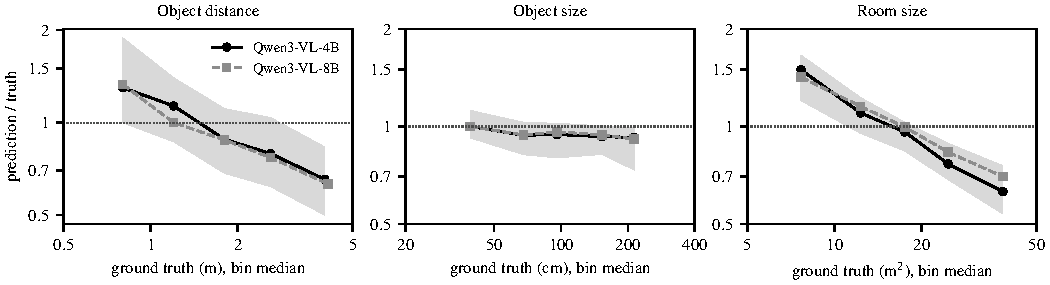
\includegraphics[width=\textwidth]{fig_compression.pdf}
\caption{Answers are compressed toward typical values. For each task, questions are binned into quintiles of the ground truth; the curves show the median ratio of prediction to truth per bin (shaded: interquartile range for Qwen3-VL-4B). A model that answers proportionally lies on the dotted line. Distances and room areas are overestimated when small and underestimated when large; object sizes are nearly proportional.}
\label{fig:compression}
\end{figure*}

\begin{table*}[t]
\centering
\small
\begin{tabular}{llrcccccccc}
\toprule
& & & \multicolumn{2}{c}{Compression slope} & \multicolumn{2}{c}{ICC} & \multicolumn{3}{c}{Variance share of $e$ (\%)} & \\
\cmidrule(lr){4-5}\cmidrule(lr){6-7}\cmidrule(lr){8-10}
Model & Task & $n$ & forward [CI] & reverse & raw & residual & bias & scene & question & LOO rescale $\Delta$ \\
\midrule
4B & Distance & 834 & 0.54 [0.48, 0.60] & 1.46 & 0.10 & 0.13 & 30 & 9 & 61 & $-$3.4 \\
4B & Object size & 953 & 0.87 [0.85, 0.90] & 1.02 & $-$0.06 & $-$0.08 & 11 & 0 & 89 & $-$8.3 \\
4B & Room size & 288 & 0.52 [0.48, 0.56] & 0.69 & -- & -- & 72 & -- & 28 & -- \\
\midrule
8B & Distance & 834 & 0.55 [0.50, 0.61] & 1.44 & 0.07 & 0.12 & 29 & 8 & 62 & $-$2.5 \\
8B & Object size & 953 & 0.90 [0.87, 0.93] & 1.06 & $-$0.03 & $-$0.04 & 6 & 0 & 94 & $-$8.9 \\
8B & Room size & 288 & 0.60 [0.57, 0.64] & 0.76 & -- & -- & 62 & -- & 38 & -- \\
\bottomrule
\end{tabular}
\caption{Scene-shared error is small; most error variance is magnitude-dependent bias (room size) or per-question error (distance, object size). Decomposition of baseline answers on all scenes. Compression slope: slope of $\log\hat y$ on $\log y$ (forward) and the reverse-regression value, which bounds the slope if all scatter were label noise. ICC: share of variance of $e$ (raw) or of its residual after removing the magnitude-dependent bias (residual) that is shared within scenes. Variance shares split the variance of $e$ into bias, scene-shared residual, and per-question residual. LOO rescale $\Delta$: change in MRA when each answer is divided by the mean error of the other questions in its scene. Room size has one question per scene, so scene effects cannot be estimated.}
\label{tab:decomp}
\end{table*}

\begin{figure*}[t]
\centering
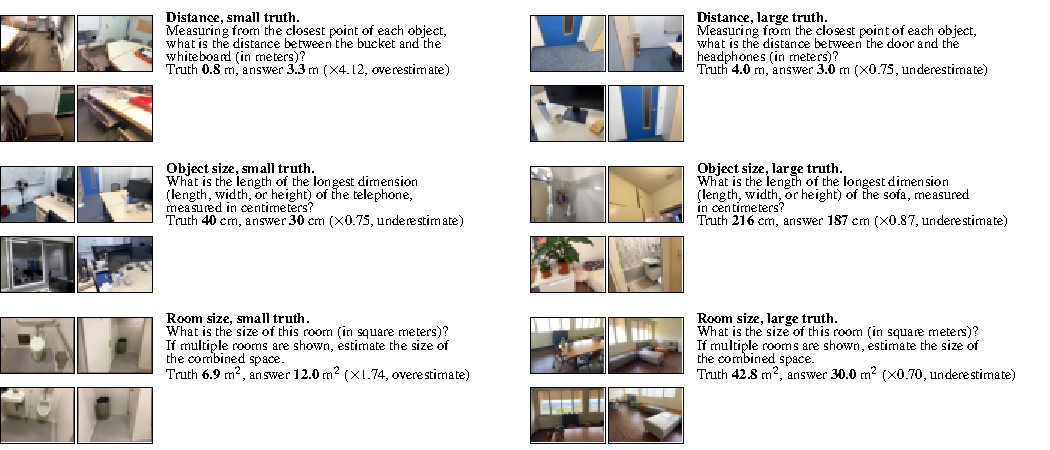
\includegraphics[width=\textwidth]{fig_qual_compression.pdf}
\caption{Small quantities are overestimated and large ones underestimated for distance and room size; object sizes stay close to the truth. Baseline answers of Qwen3-VL-4B on the evaluation questions whose ground truth is closest to the 10th (left) and 90th (right) percentile of each task, among questions answered under all conditions (four of the 16 input frames shown).}
\label{fig:qual}
\end{figure*}

\subsection{Results}

\paragraph{Answers are compressed toward typical values.}
Figure~\ref{fig:compression} and Table~\ref{tab:decomp} show that the dominant systematic error depends on the true magnitude, and Figure~\ref{fig:qual} shows examples. For Qwen3-VL-4B, the median distance answer is 1.30 times the truth for the shortest fifth of distances and 0.65 times the truth for the longest fifth; for room area the ratio falls from 1.50 to 0.63. The compression slopes are 0.54 for distance and 0.52 for room size, so answers grow roughly with the square root of the truth. Object sizes are close to proportional (slope 0.87), which fits the view that sizes of object categories are well covered by semantic priors. The answers also concentrate on a few values: the five most frequent answers cover 54\% of distance answers and 62\% of room-size answers. Qwen3-VL-8B shows the same pattern, with slopes of 0.55 (distance), 0.90 (object size), and 0.60 (room size).

\paragraph{Scene-shared error is small.}
After removing the magnitude-dependent bias, the scene-shared share of residual variance is 0.13 for distance and indistinguishable from zero for object size (Table~\ref{tab:decomp}). As a share of the total error variance, scene-shared error accounts for 9\% (distance) and 0\% (object size), against 61\% and 89\% for per-question error; the 8B model gives 8\% and 0\%. Errors are not shared across tasks either: the rank correlation between a scene's mean residual on one task and on another is $-0.07$ (distance, size), $0.24$ (distance, room), and $0.05$ (size, room). A model that misjudged the scale of a scene would err in the same direction on all three.

\paragraph{Per-scene rescaling lowers accuracy.}
The leave-one-out rescale uses ground-truth errors of other questions in the same scene and still lowers MRA, by 3.4 points for distance and 8.3 points for object size (2.5 and 8.9 for the 8B model). The global correction changes MRA by less than one point. With so little shared error, the correction mostly transfers noise from one question to another.

\paragraph{Interpretation and caveats.}
Taken together, a per-scene scale error is a minor component. Most error variance is magnitude-dependent bias (room size, 72\%) or question-specific (distance 61\%, object size 89\%). Two caveats apply. First, label noise in the ground truth biases the forward slope toward zero. The reverse-regression value bounds the true slope if all scatter came from label noise~\citep{fuller1987measurement}. For room size this bound is 0.69, so compression is robust; for distance it is 1.46, because the correlation between answers and truth is only 0.61. The compression claim for distance therefore assumes that most scatter comes from the model rather than from the labels. Second, the ICC is estimated from scenes with few questions each (about four for distance), which limits its precision; the 95\% interval of the residual ICC for distance is [0.06, 0.21], so even its upper end leaves most variance per question.

\section{Can a Scale Cue Fix the Errors?}

\subsection{Cues and controls}
We prepend one line to the question. Each cue is tested at its correct value ($k=1$) and multiplied by $k \in \{0.5, 2\}$; the depth and anchor cues of the 4B model are also tested at $k \in \{0.71, 1.41\}$. The exact wording is in the appendix.
\begin{itemize}
\item \textbf{Depth scale (teacher).} The median metric depth of the 16 frames, estimated by MapAnything~\citep{keetha2025mapanything}: ``the typical distance from the camera to visible surfaces in this video is about $X$\,m''. A variant (\emph{depth + extent}) adds the diagonal of the reconstructed point cloud, which is informative about room size (rank correlation 0.80 with the square root of room area).
\item \textbf{Learned scale.} The same depth scale predicted from the model's own pooled vision features by a small network trained on the training scenes (error vs.\ the teacher 0.095 in median absolute log, against 0.185 for a constant).
\item \textbf{Shuffled.} The depth scale of a different scene, as a control for the presence of a number.
\item \textbf{Anchor object.} The ground-truth longest dimension of a \emph{different} object in the same scene, taken from VSI-Bench's object-size questions: ``the sofa in this video is about 346\,cm along its longest dimension''. The anchor object is never named in the target question. This cue is metric and exact, so the model does not need to convert camera depth into object distances.
\item \textbf{Placebo.} A line asking the model to consider the physical scale of the scene, without a number.
\item \textbf{Answer (positive control).} ``the correct answer is approximately $X$'', with $X$ the ground truth times $k$. This tests whether the model can use a number in the prompt at all.
\end{itemize}
We also test a reasoning prompt in the style of \citet{liao2024reasoning}, which asks the model to pick reference objects of known size and use them as a ruler, with up to 512 new tokens.

We measure the use of a cue by its \emph{elasticity}: for each question we fit the slope $\beta$ of $\log \hat y$ on $\log k$ over the tested multipliers. An answer that follows the cue proportionally has $\beta = 1$; an answer that ignores it has $\beta = 0$. This is the response slope of \citet{tan2026scale}.

\begin{table}[t]
\centering
\small
\setlength{\tabcolsep}{3pt}
\begin{tabular}{lccc}
\toprule
Condition & Distance & Object size & Room size \\
\midrule
Baseline (MRA) & 44.7 & 72.8 & 50.3 \\
\midrule
Placebo & $-$0.2 & $-$0.3 & $-$0.4 \\
Shuffled & $-$0.2 & $-$0.5 & $-$0.3 \\
Depth scale & $+$0.3 & $-$0.7 & $+$1.5 \\
Depth + extent & $-$1.2 & $-$0.3 & $+$0.2 \\
Learned scale & $-$1.0 & $-$0.5 & $+$1.3 \\
Anchor object & $-$0.8 & $-$0.1 & $+$2.3 \\
Reasoning prompt & $-$10.4$^\ast$ & $-$24.6$^\ast$ & $-$19.8$^\ast$ \\
\midrule
Answer (control) & $+$20.4$^\ast$ & $+$9.7$^\ast$ & $+$49.7$^\ast$ \\
\bottomrule
\end{tabular}
\caption{Change in MRA relative to the baseline on the same evaluation questions (Qwen3-VL-4B, cues at $k=1$). $^\ast$: 95\% CI excludes zero. No scale cue changes accuracy by more than 2.3 points, and none significantly. Full intervals and all $k$ levels are in the appendix.}
\label{tab:cues}
\end{table}

\begin{figure*}[t]
\centering
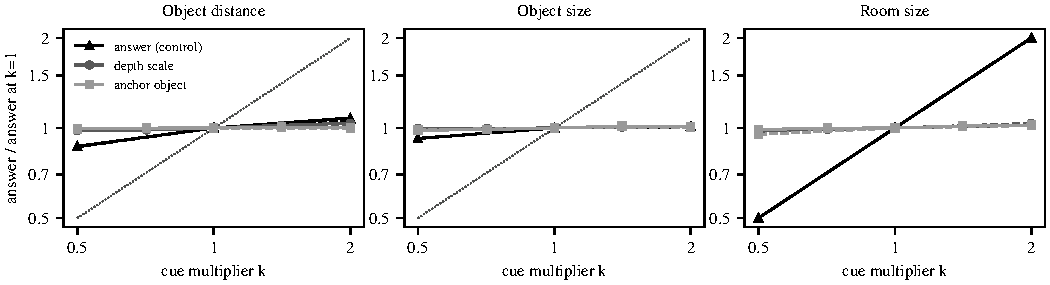
\includegraphics[width=\textwidth]{fig_elasticity.pdf}
\caption{Answers barely follow scale cues. They follow a stated answer fully for room size and only partly for distance and object size. Curves show the geometric mean ratio of the answer at cue multiplier $k$ to the answer at $k=1$ (solid: Qwen3-VL-4B, dashed: Qwen3-VL-8B). The dotted line is proportional use ($\beta=1$).}
\label{fig:elasticity}
\end{figure*}

\begin{table}[t]
\centering
\small
\setlength{\tabcolsep}{2.5pt}
\begin{tabular}{llccc}
\toprule
Cue & Task & mean $\beta$ [CI] & up / down (\%) & 8B mean $\beta$ \\
\midrule
Depth & Distance & 0.044 [0.03, 0.06] & 40 / 4 & 0.033 \\
 & Size & 0.011 [0.01, 0.02] & 24 / 8 & 0.009 \\
 & Room & 0.030 [0.02, 0.04] & 28 / 4 & 0.043 \\
Anchor & Distance & 0.006 [0.00, 0.01] & 14 / 7 & $-$0.003 \\
 & Size & 0.024 [0.02, 0.04] & 30 / 14 & 0.014 \\
 & Room & 0.025 [0.02, 0.04] & 47 / 4 & 0.049 \\
Answer & Distance & 0.157 [0.13, 0.19] & 68 / 6 & 0.149 \\
 & Size & 0.065 [0.05, 0.08] & 47 / 8 & 0.066 \\
 & Room & 1.000 [1.00, 1.00] & 100 / 0 & 1.000 \\
\bottomrule
\end{tabular}
\caption{Elasticity to scale cues is near zero; a stated answer is followed fully only for room size. Mean elasticity $\beta$ of answers with respect to the cue value (Qwen3-VL-4B unless noted). Up / down: share of questions whose answer increases / decreases from $k=0.5$ to $k=2$; the rest are unchanged. Elasticities use $k \in \{0.5, 0.71, 1, 1.41, 2\}$ for 4B scale cues and $k \in \{0.5, 1, 2\}$ otherwise.}
\label{tab:elasticity}
\end{table}

\subsection{Results}

\paragraph{No scale cue improves accuracy.}
Table~\ref{tab:cues} shows paired changes in MRA. Every scale cue changes accuracy by between $-1.2$ and $+2.3$ points, and no interval excludes zero. This includes the exact anchor size and the learned scale, and it holds for the cue that is informative about room size (depth + extent). For the 8B model, no cue improves accuracy either, and two lower it slightly: the anchor on distance ($-2.4$, CI [$-4.7$, $-0.2$]) and the depth scale on object size ($-1.3$, CI [$-2.5$, $-0.3$]); see the appendix. The reasoning prompt lowers MRA by 10--25 points; 7\% of its answers end in repetition loops that do not terminate even with 2048 tokens, but excluding them still leaves drops of 10--20 points.

\paragraph{The model registers the cue but barely uses it.}
The cue does change answers: 36--57\% of answers differ from the baseline, against 26--39\% for the placebo line, which shows that part of this change is generic sensitivity to the prompt. The change is directional. From $k=0.5$ to $k=2$, answers move up far more often than down, for example 40\% versus 4\% for the depth cue on distance (Table~\ref{tab:elasticity}). Its size, however, is tiny: the mean elasticity is 0.006--0.044 for the 4B model and $-0.003$--0.049 for the 8B model, so doubling the cue raises the answer by a few percent rather than by a factor of two (Figure~\ref{fig:elasticity}). The median elasticity is zero because most answers do not change at all between the extreme values.

\paragraph{The model can use numbers in the prompt, but trusts its own estimate.}
When the cue states the correct answer ($k=1$), MRA rises by 20.4 (distance), 9.7 (object size), and 49.7 points (room size), and by 21.5, 10.5, and 45.1 points for the 8B model, so the models read numbers in the prompt and use them. How far they follow a stated answer that is wrong by a factor of two depends on the task. For room size they copy the stated value at every $k$ (elasticity 1.00 for both models). For distance and object size they keep most of their own estimate (elasticity 0.16 and 0.07 for 4B, 0.15 and 0.07 for 8B), even though the prompt asserts what the answer is. The model thus defers to the text for room size, the task with the strongest compression, and holds on to its visual estimate for object-level quantities. Scale cues fall below even this level on every task, including room size, where the model copies a stated area but does not turn a depth or extent cue into one. This contrasts with response slopes of 0.69--0.94 reported by \citet{tan2026scale} for physics questions in which the prompt is the only source of metric information; in natural videos, the model's own estimate dominates.

\section{Why Scale Cues Cannot Help}
Low elasticity looks like a failure only if the cues carry useful information. Section~\ref{sec:where} suggests that they do not: if errors are not shared within scenes, knowing the scene's scale does little to correct an individual answer. We test this directly by asking how much accuracy an ideal user of each cue could reach, using only training scenes to fit any parameters.

\begin{table}[t]
\centering
\small
\setlength{\tabcolsep}{2pt}
\begin{tabular}{llcc}
\toprule
Task & Method & MRA & $\Delta$ vs.\ raw [CI] \\
\midrule
Distance & Oracle anchor rescale & 41.3 & $-$4.3 [$-$8.3, $-$0.7] \\
Object size & Oracle anchor rescale & 59.7 & $-$12.9 [$-$17.2, $-$8.6] \\
Room size & Oracle anchor rescale & 44.4 & $-$5.1 [$-$10.6, $-$0.1] \\
\midrule
Distance & Calibrated answer & 42.4 & $-$3.0 [$-$6.2, 0.0] \\
 & + depth scale & 42.6 & $-$2.7 [$-$6.1, 0.6] \\
Room size & Calibrated answer & 55.7 & $+$5.4 [$-$0.4, 10.8] \\
 & + scene extent & 61.4 & $+$11.0 [4.6, 17.7] \\
 & Extent in prompt & 50.5 & $+$0.2 [$-$2.5, 3.1] \\
\bottomrule
\end{tabular}
\caption{Even ideal use of the anchor lowers accuracy; only the scene extent adds information, and only for room size. Oracle anchor rescale: answer multiplied by the true anchor size divided by the model's own estimate of that anchor. Calibrated: log-linear regression of the ground truth on the model's answer (and the cue), fitted on training scenes. Qwen3-VL-4B, evaluation scenes.}
\label{tab:headroom}
\end{table}

\paragraph{The anchor cue carries no usable information.}
If the model's errors were shared within a scene, its error on the anchor object would predict its error on the target. We use the anchor in the most favorable way: we divide each answer by the model's own error on the anchor object, that is, multiply it by the true anchor size divided by the model's estimate of it. This \emph{lowers} MRA on every task (Table~\ref{tab:headroom}). Ignoring the anchor is therefore the right behavior for this model, and its low elasticity is not a missed opportunity.

\paragraph{The depth cue carries little information about distances.}
A log-linear calibration of the model's distance answers, fitted on training scenes, lowers distance accuracy by 3.0 points, and adding the depth scale as a second predictor changes the calibrated result by only $+0.3$ points (CI [$-1.0$, $1.6$]). Distance errors are mostly per-question noise, which no scene-level quantity can remove.

\paragraph{Room size is the exception.}
For room size, where most error variance is magnitude-dependent bias, two things help. A two-parameter recalibration of the model's own answers raises MRA by 5.4 points (CI [$-0.4$, $10.8$]), because it undoes the compression. Adding the scene extent from the 3D reconstruction raises it by 11.0 points in total; the extent's contribution beyond recalibration is 5.7 points (CI [1.7, 10.2]). The same extent written into the prompt changes MRA by 0.2 points. Here the model ignores information that a simple post-hoc combination exploits. The gain comes from a calibrated combination of the answer and the extent outside the model, not from a cue that the model reads.

\section{Discussion}

\paragraph{What to invest in.}
Our results separate three regimes. Object size errors are small and nearly proportional; semantic priors already work. Room size errors are mostly compression; recalibrating the output and combining it with a geometric extent estimate raises accuracy by 11 points, without changing the model. Distance errors are mostly per-question: they reflect where the model localizes the two objects and how it measures between them, and no single number per scene can fix them. Methods that improve distance therefore have to improve per-question grounding and geometry. This is consistent with the large gains of tool-based pipelines that measure each distance explicitly~\citep{glantz2026seeing}, and it suggests that such gains are unlikely to come from supplying scene scale alone.

\paragraph{Compression as central tendency.}
The compression we observe has the signature of central tendency in human magnitude estimation~\citep{hollingworth1910central,jazayeri2010temporal}: when evidence is weak, estimates shrink toward the prior mean. The frequent repetition of a few answers points the same way, as does the models' readiness to copy a stated room area while keeping their own estimate against a stated distance. This reading predicts that compression should be strongest where visual evidence is weakest, which matches the near-proportional answers for object size, a task with strong category priors and direct visual evidence.

\paragraph{Limitations.}
We study two models of one family, on indoor videos, with cues given as text. Visual or token-level cues may be used differently. We give frames as images rather than as video and run in bfloat16; both choices are fixed across conditions but differ from the official protocol. The compression slope for distance depends on the assumption that label noise is small relative to model noise. The learned scale, the teacher, and the calibrations use only training scenes, but the anchor cue uses benchmark labels by design.

\section{Conclusion}
The metric errors of frozen Qwen3-VL models on VSI-Bench are not mainly errors of scene scale. They consist of compression toward typical values and per-question error, and errors shared within a scene are small. As a consequence, scale cues, including exact ones, do not improve accuracy, and for most cues giving them little weight costs nothing; only for room size does a cue carry information that the model leaves unused. We suggest that evaluations of new metric reasoning methods report the error decomposition alongside accuracy, so that it becomes clear which component a method removes.

\bibliography{refs}

\appendix

\section{Prompts}
All conditions use the benchmark question followed by ``Please answer the question using a single word or phrase.'' The cue line is placed before the question:
\begin{itemize}
\item Depth scale: ``Scale reference: the typical distance from the camera to visible surfaces in this video is about $X$ m.'' (depth + extent appends ``The scene spans about $E$ m.'')
\item Anchor: ``Scale reference: the $\langle$object$\rangle$ in this video is about $X$ cm along its longest dimension.''
\item Placebo: ``Scale reference: consider the physical scale of the scene carefully.''
\item Answer: ``Hint: the correct answer is approximately $X$ $\langle$unit$\rangle$.''
\item Reasoning prompt: ``Before answering, pick one or more reference objects in the video whose real-world size you know well, estimate their size, and use them as a ruler to measure what is asked.'', with the instruction ``Think step by step, then end your reply with a line of the form `Final answer: $\langle$number$\rangle$'.'' Only the text after ``Final answer'' is parsed when present.
\end{itemize}

\section{Implementation Details}
\paragraph{Teacher.} MapAnything (Apache-licensed weights) runs on the same 16 frames resized to a longest side of 336 pixels in bfloat16. It succeeded on all 288 scenes. The median depth over valid pixels is the depth scale; the diagonal of the 5--95 percentile box of the point cloud is the extent.
\paragraph{Learned scale.} Vision tokens of Qwen3-VL-4B are mean-pooled per frame ($16 \times 2560$). A ridge probe (2.6K parameters) and a two-layer frame transformer (1.75M parameters) predict the log depth scale; the transformer was chosen on 17 held-out training scenes (validation error 0.054 vs.\ 0.080) although the ridge probe is better on evaluation scenes (0.083 vs.\ 0.095). Training takes 22\,s for three seeds.
\paragraph{Anchor table.} For each question we take, in order of question ID, the first object-size question of the same scene whose object is not named in the target question. This covers 788 of 836 evaluation questions; changes in MRA are paired on these questions.
\paragraph{Reasoning prompt.} 22 of 300 answers (17 on object size) did not reach a final answer within 512 tokens. Rerunning them with 2048 tokens showed that all 22 are repetition loops, so we keep the 512-token run. Without these answers, the changes in MRA are $-10.4$, $-18.7$, and $-19.6$ points.
\paragraph{Compute.} All runs used one NVIDIA RTX 5090 in bfloat16; a full condition takes about 12 minutes for the 4B model.

\section{Random Examples}
Figure~\ref{fig:random} shows nine evaluation questions drawn at random (seed 0, three per task) from those answered under all conditions, to show that the examples in Figure~\ref{fig:teaser} are typical.

\begin{figure*}[t]
\centering
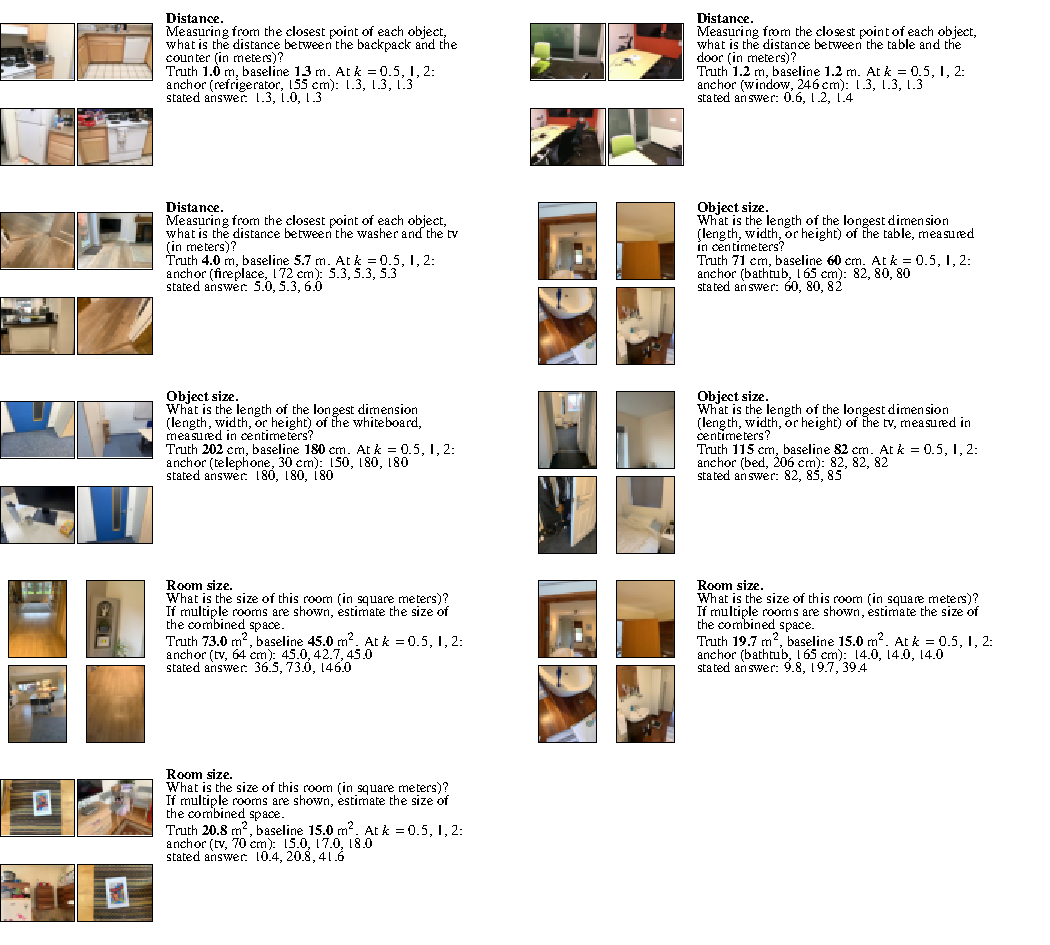
\includegraphics[width=\textwidth]{fig_qual_random.pdf}
\caption{Randomly drawn examples (Qwen3-VL-4B). Under the anchor cue the answer changes little across $k$; a stated answer is copied for room size and followed only partly for distance and object size.}
\label{fig:random}
\end{figure*}

\section{Full Results}
Table~\ref{tab:full} lists the paired change in MRA for every condition, model, and cue multiplier. The answer control at $k \ne 1$ lowers accuracy sharply for room size, where the model copies the wrong value, and only mildly for distance and object size, where it mostly keeps its own estimate.

\begin{table*}[t]
\centering
\small
\begin{tabular}{lccc}
\toprule
Condition & Distance & Object size & Room size \\
\midrule
\multicolumn{4}{l}{\emph{Qwen3-VL-4B}, baseline MRA: 44.7, 72.8, 50.3} \\
placebo & $-$0.2 [$-$1.8, 1.1] & $-$0.3 [$-$1.4, 0.8] & $-$0.4 [$-$2.4, 1.5] \\
reasoning & $-$10.4 [$-$17.3, $-$3.8] & $-$24.6 [$-$32.2, $-$16.8] & $-$19.8 [$-$29.1, $-$10.4] \\
shuffled & $-$0.2 [$-$2.0, 1.8] & $-$0.5 [$-$1.5, 0.5] & $-$0.3 [$-$3.0, 2.3] \\
learned & $-$1.0 [$-$2.9, 0.7] & $-$0.5 [$-$1.4, 0.3] & $+$1.3 [$-$1.8, 5.2] \\
depth + extent & $-$1.2 [$-$4.2, 1.4] & $-$0.3 [$-$1.4, 0.7] & $+$0.2 [$-$2.5, 3.1] \\
depth $k$=0.5 & 0.0 [$-$1.5, 1.5] & $-$1.0 [$-$1.9, $-$0.1] & $+$0.0 [$-$3.3, 3.7] \\
depth $k$=0.71 & $+$1.0 [$-$0.7, 2.8] & $-$0.8 [$-$1.8, 0.0] & $+$0.7 [$-$2.3, 4.4] \\
depth & $+$0.3 [$-$1.3, 2.0] & $-$0.7 [$-$1.7, 0.2] & $+$1.5 [$-$1.6, 4.7] \\
depth $k$=1.41 & $+$0.1 [$-$1.6, 1.8] & $-$0.3 [$-$1.3, 0.6] & $+$0.6 [$-$1.8, 3.2] \\
depth $k$=2 & $-$0.4 [$-$2.3, 1.7] & $-$0.2 [$-$1.2, 0.7] & $-$0.3 [$-$2.4, 1.7] \\
anchor $k$=0.5 & $-$1.8 [$-$3.9, 0.2] & $-$1.8 [$-$3.1, $-$0.8] & $+$1.7 [$-$0.8, 4.2] \\
anchor $k$=0.71 & $-$1.6 [$-$3.6, 0.4] & $-$1.5 [$-$2.8, $-$0.4] & $+$2.2 [$-$0.5, 4.9] \\
anchor & $-$0.8 [$-$3.1, 1.7] & $-$0.1 [$-$1.3, 0.9] & $+$2.3 [$-$0.7, 5.3] \\
anchor $k$=1.41 & $-$0.5 [$-$2.6, 1.4] & $-$0.2 [$-$1.3, 1.0] & $+$2.6 [$-$0.6, 5.3] \\
anchor $k$=2 & $-$1.0 [$-$3.2, 1.1] & $-$0.2 [$-$1.5, 1.1] & $+$3.4 [0.3, 6.4] \\
answer $k$=0.5 & $-$8.0 [$-$10.9, $-$4.9] & $-$3.4 [$-$5.4, $-$1.7] & $-$42.5 [$-$48.6, $-$36.6] \\
answer & $+$20.4 [17.2, 23.9] & $+$9.7 [7.9, 11.5] & $+$49.7 [43.5, 55.9] \\
answer $k$=2 & $-$5.6 [$-$8.3, $-$3.1] & $-$1.8 [$-$3.6, $-$0.2] & $-$50.3 [$-$56.2, $-$44.1] \\
\midrule
\multicolumn{4}{l}{\emph{Qwen3-VL-8B}, baseline MRA: 44.4, 72.5, 54.9} \\
placebo & $-$1.5 [$-$3.0, 0.0] & $+$0.1 [$-$1.1, 1.1] & $+$1.4 [$-$1.4, 4.2] \\
depth $k$=0.5 & $-$2.8 [$-$4.7, $-$0.8] & $-$1.1 [$-$2.0, $-$0.2] & $+$0.3 [$-$3.7, 4.3] \\
depth & $-$0.9 [$-$3.0, 1.0] & $-$1.3 [$-$2.5, $-$0.3] & $+$0.0 [$-$3.3, 3.1] \\
depth $k$=2 & $-$1.6 [$-$3.4, 0.0] & $-$0.7 [$-$2.1, 0.4] & $+$0.4 [$-$2.4, 3.2] \\
anchor $k$=0.5 & $-$2.9 [$-$5.2, $-$0.6] & $-$2.0 [$-$3.0, $-$0.9] & $+$1.7 [$-$2.0, 5.6] \\
anchor & $-$2.4 [$-$4.7, $-$0.2] & $-$0.5 [$-$1.7, 0.7] & $+$2.2 [$-$1.3, 5.5] \\
anchor $k$=2 & $-$2.5 [$-$4.6, $-$0.3] & $-$0.7 [$-$2.1, 0.6] & $+$0.9 [$-$2.1, 4.1] \\
answer $k$=0.5 & $-$7.9 [$-$11.0, $-$4.9] & $-$3.9 [$-$6.3, $-$1.8] & $-$47.0 [$-$52.3, $-$40.9] \\
answer & $+$21.5 [17.9, 25.3] & $+$10.5 [8.3, 12.7] & $+$45.1 [39.6, 50.7] \\
answer $k$=2 & $-$3.3 [$-$6.2, $-$0.8] & $-$2.8 [$-$5.2, $-$0.9] & $-$54.9 [$-$60.5, $-$48.9] \\
\bottomrule
\end{tabular}
\caption{Paired change in MRA relative to the baseline on the same evaluation questions, with 95\% scene-bootstrap intervals, for every condition. ``depth'' is the teacher depth scale; ``reasoning'' is the reference-object reasoning prompt.}
\label{tab:full}
\end{table*}

\end{document}
